\chapter{ANÁLISE DOS RESULTADOS}\label{ch:conclusao}

Este capítulo tem como finalidade apresentar os resultados obtidos através das implementações demonstrados no Capítulo~\ref{ch:implementacao}.

\section{APRESENTAÇÃO DOS RESULTADOS}

Após o mapeamento das informações do \textit{DataFrame} foi construído um gráfico em barras indicando as quantidades de \textit{tweets} em relação aos quatro idiomas mais significativos no conjunto de dados coletados, Gráfico~\ref{lingua}.

\begin{grafico}[h]
	\centering
	\fbox{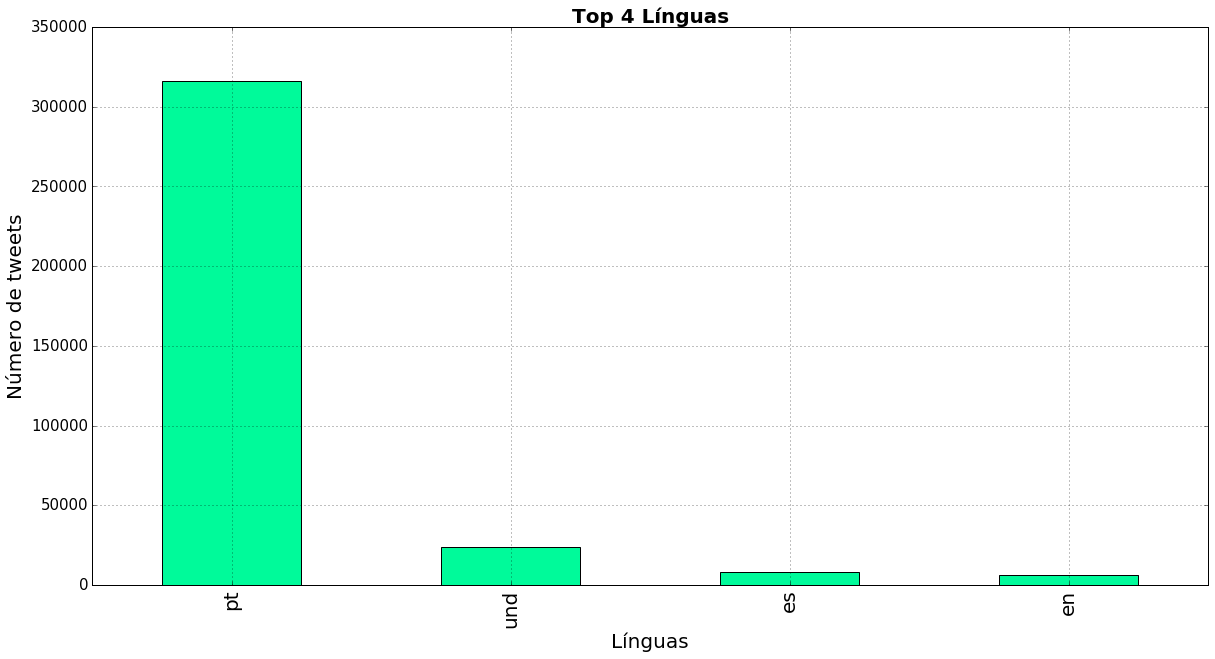
\includegraphics[width=1\textwidth]{Cap5/graficos/linguas}}
	\caption{Idiomas que mais realizaram \textit{tweets}}
	\vspace{-0.3cm}
	\legend{FONTE: Elaborado pelo autor}
	\label{lingua}
\end{grafico}

É possível verificar nesta figura que existe uma barra com o nome de \textit{und} para especificar o segundo idioma que mais realizou \textit{tweets}. Essa é uma condição em que não foi identificado o idioma de origem e, então, a API do \textit{Twitter} classifica como \textit{undefined}, ou indefinido no português. Essa linguagem indefinida ocorre devido ao \textit{software} em que o usuário está realizando o \textit{tweet}, por exemplo; um navegador \textit{web}, um aplicativo \textit{mobile} do \textit{Twitter} ou algum aplicativo de terceiro que permite realizar ações no \textit{Twitter}. Caso a linguagem não esteja definida nestes ambientes, a API a classifica como indefinida \cite{twitter-doc}.


O Código~\ref{map-pais} verifica quais são os cinco países que mais realizaram \textit{tweets} através do mapeamento do \textit{DataFrame} e constrói um gráfico em barras para representá-los, Gráfico~\ref{paises}.

\begin{grafico}[h]
	\centering
	\fbox{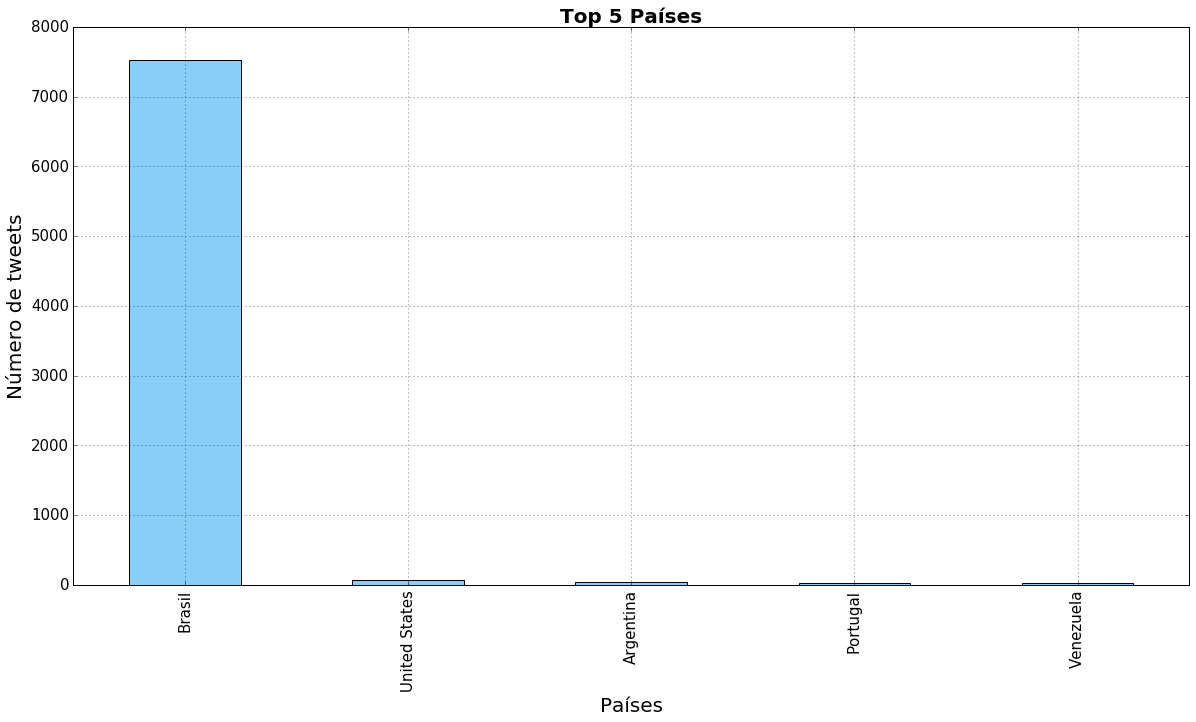
\includegraphics[width=1\textwidth]{Cap5/graficos/paises}}
	\caption{Países que mais realizaram \textit{tweets}}
	\vspace{-0.3cm}
	\legend{FONTE: Elaborado pelo autor}
	\label{paises}
\end{grafico}

Este gráfico demonstra, claramente, que a maior número de \textit{tweets} foram publicados do Brasil e apenas uma pequena quantia deles foram realizados nos Estados Unidos, Argentina, Portugal e Venezuela. É importante notar que nem todos os \textit{tweets} gerados possuem um país de origem, o que se assemelha a situação anterior, onde a API do \textit{Twitter} os classifica como \textit{undefined}, porém não sendo apresentado no gráfico da Figura~\ref{paises}.

As \textit{hashtags} são contabilizadas e apresentadas através do gráfico de setores da Figura~\ref{hashtag}, onde é possível verificar a porcentagem referente aos \textit{tweets} realizados com a \textit{hashtag} \#ImpeachmentDay. 

\begin{grafico}[h]
	\centering
	\fbox{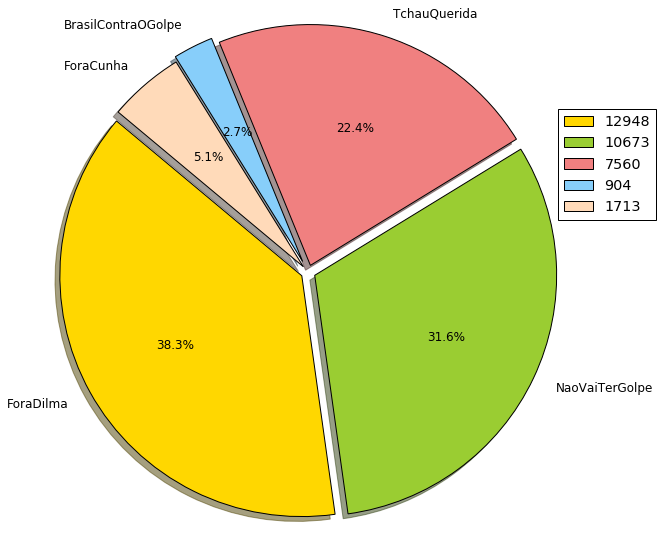
\includegraphics[width=1\textwidth]{Cap5/graficos/hashtag}}
	\caption{\textit{Hashtags} com o maior número de \textit{tweets}}
	\vspace{-0.3cm}
	\legend{FONTE: Elaborado pelo autor}
	\label{hashtag}
\end{grafico}

Através do Gráfico~\ref{hashtag}, pode-se notar que as \textit{hashtags} \#ForaDilma e \#TchauQuerida somaram um total de 60,7\%, indicando que a maioria dos \textit{tweets} eram de apoio ao processo de Impeachment da Presidente da República, diferentemente dos 34,3\% dos \textit{tweets} que é o somatório de \#BrasilContraOGolpe e \#NaoVaiTerGolpe.

Como resultado, o Código~\ref{cod-fig-pol} constrói um gráfico em setores, onde é possível verificar a porcentagem de \textit{tweets} para nomes específicos, Gráfico~\ref{fig-pol}, porém não é possível, ainda, predizer se os argumentos a respeito destas pessoas são positivos ou negativos.

\begin{grafico}[h]
	\centering
	\fbox{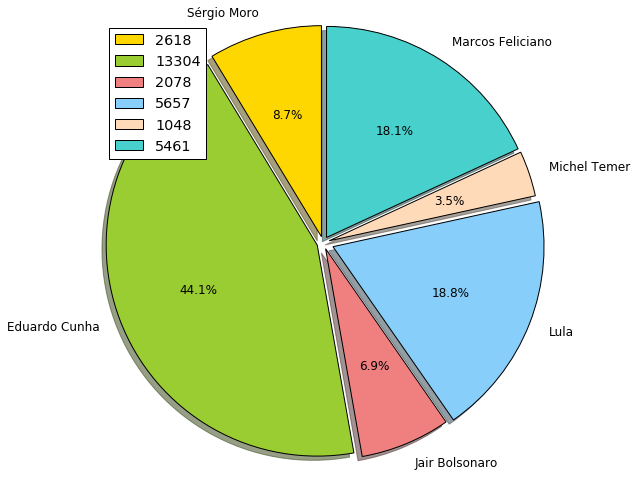
\includegraphics[width=1\textwidth]{Cap5/graficos/figuras-politicas}}
	\caption{Gráfico em setores para figuras importantes}
	\vspace{-0.3cm}
	\legend{FONTE: Elaborado pelo autor}
	\label{fig-pol}
\end{grafico}

O gráfico de setores representado pela Figura~\ref{fig-pol}, demonstra que o nome mais mencionado foi de Eduardo Cunha e com apenas 2618 \textit{tweets} o nome de Michel Temer foi publicado. Até mesmo as menções ao ex-presidente Luiz Inácio "Lula" da Silva recebeu apenas 18,8\% do total dos nomes filtrados.


